\documentclass[bluish,slideColor,colorBG,pdf]{prosper}
\hypersetup{pdfpagemode=FullScreen}
\usepackage{graphicx,amsfonts,amsmath}
\usepackage{bm}
\def\baselinestretch{1.0}
\setlength{\topmargin}{-60pt}
\setlength{\textheight}{460pt}
\setlength{\oddsidemargin}{0pt}
\setlength{\evensidemargin}{0pt}
\setlength{\textwidth}{660pt}
\setlength{\footskip}{0pt}
\parindent 0.3in
\hyphenpenalty=10000
\tolerance=10000
\pagestyle{empty}

\def\Prob{{\rm Prob\;}}
\def\prob{{\rm \;Prob\;}}
\def\Var{{\rm Var}}        % Var
\def\Cov{{\rm Cov}}        % Cov

\DeclareSymbolFont{AMSb}{U}{msb}{m}{n}
\DeclareMathSymbol{\expect}{\mathalpha}{AMSb}{'105}

\title{Week 5:  Distance methods, DNA and protein models}
\author{Genome 570}
\institution{February, 2016}

\begin{document}

\maketitle

\bigskip

\begin{slide}[Replace]{A tree and the expected distances it predicts}

\centerline{\includegraphics[width=4in]{fig11-1.ydraw}}
\bigskip

The predicted distances are the sums of branch lengths between those two
species.

\end{slide}

\begin{slide}[Replace]{A tree and a set of two-species trees}
\bigskip

\centerline{\includegraphics[width=3.5in]{twospecies.ydraw}}
\bigskip

The two-species trees correspond to the pairwise distances
observed between the pairs of species.  The tree also predicts
two-species trees, because clipping off all other species you are
left simply with the path between that pair of species.

\end{slide}

\begin{slide}[Replace]{A tree with branch lengths}
\bigskip

\centerline{\includegraphics[width=2.4in]{fig11-2.ydraw}}
\bigskip

Distance matrix methods always infer trees that have branch lengths, and they
assume models of change of the characters (sequences).

\end{slide}

\begin{slide}[Replace]{Distance matrix methods}

\vspace{-0.1in}
\hspace*{0in}\hspace{-0.3in}\centerline{\includegraphics[width=3.1in]{distmatrix.idraw}}

\end{slide}

\begin{slide}[Replace]{The math of least squares trees}

\[
\mathsf{Q \ =\  \sum_{i=1}^n \sum_{j \neq i}  w_{ij} (D_{ij}-d_{ij})^2}
\]

\[
\mathsf{d_{ij}\  =\  \sum\limits_k x_{ij,k} v_k}
\]

\[
\mathsf{Q\  =\  \sum_{i=1}^n \sum_{j \neq i}  w_{ij} \left(D_{ij}-\sum\limits_k x_{ij,k} v_k\right)^2.  }
\]

\[
\mathsf{\frac{dQ}{dv_k}\  =\  -2 \sum_{i=1}^n \sum_{j \neq i}  w_{ij}\; x_{ij,k} \left(D_{ij}-\sum\limits_k x_{ij,k} v_k\right)\  =\  0.}
\]

Equations to solve to infer branch lengths by least squares on a given tree
topology, which specifies the $\ \mathsf{x_{ij,k}}$.

\end{slide}

\begin{slide}[Replace]{Solving for least squares branch lengths}

\[
\begin{array}{l c l}
\mathsf{D_{AB} + D_{AC} + D_{AD} + D_{AE}} & \mathsf{=} & \mathsf{4 v_1 + v_2 + v_3 + v_4 + v_5 + 2 v_6 + 2 v_7}\\
\mathsf{D_{AB}+D_{BC}+D_{BD}+D_{BE}}& \mathsf{=} & \mathsf{v_1 + 4 v_2 + v_3 + v_4 + v_5 + 2 v_6 + 3 v_7}\\
\mathsf{D_{AC} + D_{BC} + D_{CD} + D_{CE}} & \mathsf{=} & \mathsf{v_1 + v_2 + 4 v_3 + v_4 + v_5 + 3 v_6 + 2 v_7}\\
\mathsf{D_{AD} + D_{BD} + D_{CD} + D_{DE}} & \mathsf{=} & \mathsf{v_1 + v_2 + v_3 + 5 v_4 + v_5 + 2 v_6 + 3 v_7}\\
\mathsf{D_{AE} + D_{BE} + D_{CE} + D_{DE}} & \mathsf{=} & \mathsf{v_1 + v_2 + v_3 + v_4 + 4 v_5 + 3 v_6 + 2 v_7}\\
\mathsf{D_{AC}+D_{AE} + D_{BC}} & & \\
\mathsf{\ + D_{BE} + D_{CD} + D_{DE}} & \mathsf{=} & \mathsf{2 v_1 + 2 v_2 + 3 v_3 + 2 v_4 + v_5 + 6 v_6 + 4 v_7}\\
\mathsf{D_{AB}+D_{AD}+D_{BC}}\\
\mathsf{\ + D_{BE} + D_{CD} + D_{DE}} & \mathsf{=} & \mathsf{2 v_1 + 3 v_2 + 3 v_4 + 2 v_5 + 4 v_6 + 6 v_7}
\end{array}
\]

\end{slide}

\begin{slide}[Replace]{A vector of all distances, stacked}

\[
\mathsf{d\  =\  \left[
\begin{array}{c}
\mathsf{D_{AB}}\\
\mathsf{D_{AC}}\\
\mathsf{D_{AD}}\\
\mathsf{D_{AE}}\\
\mathsf{D_{BC}}\\
\mathsf{D_{BD}}\\
\mathsf{D_{BE}}\\
\mathsf{D_{CD}}\\
\mathsf{D_{CE}}\\
\mathsf{D_{DE}}
\end{array}
\right]
}\]
\bigskip

They are in lexicographic (dictionary) order.

\end{slide}

\begin{slide}[Replace]{The design matrix and least squares equations}

\[
\mathsf{X\  =\  \left[
\begin{array}{c c c c c c c}
1 & 1 & 0 & 0 & 0 & 0 & 1 \\
1 & 0 & 1 & 0 & 0 & 1 & 0 \\
1 & 0 & 0 & 1 & 0 & 0 & 1 \\
1 & 0 & 0 & 0 & 1 & 1 & 0 \\
0 & 1 & 1 & 0 & 0 & 1 & 1 \\
0 & 1 & 0 & 1 & 0 & 0 & 0 \\
0 & 1 & 0 & 0 & 1 & 1 & 1 \\
0 & 0 & 1 & 1 & 0 & 1 & 1 \\
0 & 0 & 1 & 0 & 1 & 0 & 0 \\
0 & 0 & 0 & 1 & 1 & 1 & 1
\end{array}
\right]
}\]

\[
\mathsf{\mathsf{X}^T {\bf D}\  =\  \left(X^T X\right)\;v.}
\]

So solution of equations is

\[
\mathsf{v \ = \ (X^T X)^{-1}\;X^T {\bf D}}
\]

\end{slide}

\begin{slide}[Replace]{A diagonal matrix of weights}

\[
\mathsf{W \ = \ \left[
\begin{array}{c c c c c c c c c c}
\mathsf{w_{AB}} & 0 & 0 & 0 & 0 & 0 & 0 & 0 & 0 & 0 \\
0 & \mathsf{w_{AC}} & 0 & 0 & 0 & 0 & 0 & 0 & 0 & 0 \\
0 & 0 & \mathsf{w_{AD}} & 0 & 0 & 0 & 0 & 0 & 0 & 0 \\
0 & 0 & 0 & \mathsf{w_{AE}} & 0 & 0 & 0 & 0 & 0 & 0 \\
0 & 0 & 0 & 0 & \mathsf{w_{BC}} & 0 & 0 & 0 & 0 & 0 \\
0 & 0 & 0 & 0 & 0 & \mathsf{w_{BD}} & 0 & 0 & 0 & 0 \\
0 & 0 & 0 & 0 & 0 & 0 & \mathsf{w_{BE}} & 0 & 0 & 0 \\
0 & 0 & 0 & 0 & 0 & 0 & 0 & \mathsf{w_{CD}} & 0 & 0 \\
0 & 0 & 0 & 0 & 0 & 0 & 0 & 0 & \mathsf{w_{CE}} & 0 \\
0 & 0 & 0 & 0 & 0 & 0 & 0 & 0 & 0 & \mathsf{w_{DE}} \\
\end{array}
\right],
}\]

\end{slide}

\begin{slide}[Replace]{Weighted least squares equations}

{\large
\[
\mathsf{X^T W D\ =\ \left(X^T W X\right) v,}
\]

\[
\mathsf{v\ =\ \left(X^T W X\right)^{-1} X^T W D.}
\]
}
\bigskip

These matrix equations solve for weighted least squares estimates of the branch
lengths on a given tree.  The tree topology is specified by the design matrix
$\mathsf{\bm{X}}$ and the weights are the elements of the diagonal matrix $\mathsf{\bm
W}$.

\end{slide}

\begin{slide}[Replace]{A statistical justification for least squares}

\[
\mathsf{SSQ\  =\   \sum_{i=1}^n \sum_{j \neq i} \frac{\left(D_{ij} - \expect\left(D_{ij}\right)\right)^2} {\Var\left(D_{ij}\right)}.}
\]
\bigskip

This least squares method
\begin{itemize}
\item ... is what we would get by standard statistical least squares approaches
{\it if} the distances were normally distributed, independently varying, and
had expectation and variance as shown
\item ... but they actually aren't independent in almost all cases (such
as molecular sequences), but ...
\item ... it can be shown that the estimate of the tree will be a consistent
estimate in the case of non-independence, just not as efficient
\end{itemize}

\end{slide}


\begin{slide}[Replace]{The Jukes-Cantor model}

\centerline{\includegraphics[width=2.2in]{fig11-3.ydraw}}
\bigskip

The simplest and most symmetrical of models of DNA evolution.  In a small
interval of time $\ \mathsf{dt}\ $ the probability of change at a site is
$\ \mathsf{u\,dt}$, \ and it is equally likely to go to each of the other three
bases.

\end{slide}

\overlays{4}{
\begin{slide}[Replace]{A simple derivation of the probabilities of net change}
\bigskip

\begin{itemstep}
\item  Imagine a (fictional) kind of event that could change the base to one
of the four possible bases (including the same base) with equal probability
(instead of changing to one of the other three).
\item If you set the probability of change in that model to
$\ \mathsf{\frac{4}{3}u\,dt}$, \ it would be indistinguishable from the actual
Jukes-Cantor model.
\item If any nonzero number of these fictional events occur on a branch, the
probability of ending up with (say) base C is $\mathsf{\frac{1}{4}}$.
\item The number of these events that occur in a branch has Poisson
distribution with expected number $\mathsf{\frac{4}{3}u\,t}$, so the probability of no event is
$\mathsf{e^{-\frac{4}{3}ut}}$
\end{itemstep}

\end{slide}
}

\begin{slide}[Replace]{The Jukes-Cantor model}

\noindent
\hspace*{0in}\hspace{-0.08in}\begin{tabular}{l l}
Probability of no event:  & $\mathsf{e^{-\frac{4}{3}ut}}$  \\
Probability of some event:  & $ \mathsf{1-e^{-\frac{4}{3}ut}}$ 
\end{tabular}
\medskip

\noindent
Probability of changing to C given start at A, have rate $u$, time $t$:
\[
\mathsf{\prob(C|A, u, t)\   = \  \frac{1}{4}\left(1-e^{-\frac{4}{3}ut}\right)}
\]
fraction of sites different:
\[
\mathsf{f_D \ = \ \frac{3}{4}\left(1-e^{-\frac{4}{3}ut}\right).}
\]
Solving, the distance as function of the fraction of sites different is
\[
\mathsf{D\  =\  \widehat{ut} \  =\   - \frac{3}{4}\ln \left(1 - \frac{4}{3}f_D\right)}
\]

\end{slide}

\begin{slide}[Replace]{Fraction of sites different versus branch length}

\centerline{\includegraphics[width=4in]{fig11-4.ydraw}}
\bigskip

... as predicted by the Jukes-Cantor model.

\end{slide}

\begin{slide}[Replace]{Branch length versus fraction of sites different}

\centerline{\includegraphics[height=3in]{fig11-4a.ydraw}}

\end{slide}

\begin{slide}[Replace]{If you don't correct for multiple changes}
\bigskip

\centerline{\includegraphics[width=4in]{fig11-5.ydraw}}

\centerline{The true (unrooted) tree  \hspace{1in}  What we estimate}
\bigskip

This happening because the long path between A and C is shortened more,
proportionally, than the shorter paths between A and B and between C and B.
The only way to do this is to put in a spurious branch leading to B.
\medskip

In effect, there is a ``war'' between the long paths and the short paths.
\medskip

With properly corrected distances, each path approaches its true length
when we look at a very large number of sites.

\end{slide}

\begin{slide}[Replace]{Least squares methods}
\bigskip

These are just differently weighted least squares methods, as mentioned
previously.
\bigskip

Fitch and Margoliash (1967) used a weight of  $\mathsf{1 / D_{ij}^2}$, so
the quantity to be minimized is
\[
\mathsf{Q \ = \  \sum\limits_{ij} \frac{\left(D_{ij} - d_{ij}\right)^2}{D_{ij}^2}}
\]
\medskip

Cavalli-Sforza and Edwards (1967) used the unweighted least squares
method:
\[
\mathsf{Q \ = \ \sum\limits_{ij} \left(D_{ij} - d_{ij}\right)^2}
\]

These amount to different assumptions about the how the size of a distance
will affect its variance.

\end{slide}

\begin{slide}[Replace]{The Minimum Evolution method}
\bigskip

Kidd and Sgaramella-Zonta (1971) and (independently) Rzhetsky and Nei (1992ff.)
came up with this method:

\begin{itemize}
\item Search through tree space as usual
\item For each tree estimate branch lengths by least squares, not allowing
negative branch lengths
\item Then actually evaluate the tree {\it not} by the sum of squares,
but by the total sum of branch lengths.
\end{itemize}

This does fairly well, in spite of the mixture of two optimization
criteria.
\bigskip

Note that it is {\it not} directly related to parsimony, in spite of its name.

\end{slide}

\begin{slide}[Replace]{The UPGMA algorithm}
\vspace{-0.2in}

\centerline{\includegraphics[width=3.7in]{fig11-21.ydraw}}

Note that the weighting in effect weights each of the original tips
equally, so that a group's distance to an outside species or another group
is the average of all the distances between species in one and species in
the other.  This is a natural ``unweighted'' choice.

\end{slide}

\begin{slide}[Replace]{Sarich 1969, immunological distances}
\bigskip

\noindent
\[
\renewcommand{\arraystretch}{1.2}
\hspace*{0in}\hspace{-0.3in}\mathsf{\begin{array}{c l || c c c  c  c  c  c c}
   &        &           &            &               &              &               &                   &           &            \\
   &        & {\rm dog} & {\rm bear} & {\rm raccoon} & {\rm weasel} & {\rm seal} & {\rm sea~lion} & {\rm cat} & {\rm monkey}\\
\hline
\hline
 & {\rm dog}     &    0 & 32 & 48 & 51 & 50 & 48 & 98 &148\\
 & {\rm bear}    &   32 &  0 & 26 & 34 & 29 & 33 & 84 &136\\
 & {\rm raccoon} &   48 & 26 &  0 & 42 & 44 & 44 & 92 &152\\
 & {\rm weasel}  &   51 & 34 & 42 &  0 & 44 & 38 & 86 &142\\
~~ & {\rm seal}    &   50 & 29 & 44 & 44 &  0 & 24 & 89 & 142\\
 & {\rm sea~lion}&  48 & 33 & 44 & 38 & 24 &  0 & 90 & 142\\
 & {\rm cat}     &   98 & 84 & 92 & 86 &  89 &  90 &  0 &148\\
 & {\rm monkey}  &  148 &136 &152 &142 & 142 & 142 &148 &  0
\end{array}
}\]

\end{slide}

\begin{slide}[Replace]{Find smallest element, its rows, columns}
\bigskip

\[
\renewcommand{\arraystretch}{1.2}
\hspace*{0in}\hspace{-0.3in}\mathsf{\begin{array}{c l || c c c  c | c | c | c c}
   &        &           &            &               &              &        *       &   *                &           &            \\
   &        & {\rm dog} & {\rm bear} & {\rm raccoon} & {\rm weasel} & {\rm \bf seal} & {\rm \bf sea~lion} & {\rm cat} & {\rm monkey}\\
\hline
\hline
 & {\rm dog}     &    0 & 32 & 48 & 51 & \textcolor{purple}{\bf 50} & \textcolor{purple}{\bf 48} & 98 &148\\
 & {\rm bear}    &   32 &  0 & 26 & 34 & \textcolor{purple}{\bf 29} & \textcolor{purple}{\bf 33} & 84 &136\\
 & {\rm raccoon} &   48 & 26 &  0 & 42 & \textcolor{purple}{\bf 44} & \textcolor{purple}{\bf 44} & 92 &152\\
 & {\rm weasel}  &   51 & 34 & 42 &  0 & \textcolor{purple}{\bf 44} & \textcolor{purple}{\bf 38} & 86 &142\\
\hline
~*& \textcolor{purple}{\rm \bf seal}    &   \textcolor{purple}{\bf 50} & \textcolor{purple}{\bf 29} & \textcolor{purple}{\bf 44} & \textcolor{purple}{\bf 44} &  \textcolor{purple}{\bf 0} & \textcolor{red}{\fbox{\bf 24}} & \textcolor{purple}{\bf 89} &\textcolor{purple}{\bf 142}\\
\hline
~*& \textcolor{purple}{\rm \bf sea~lion}&  \textcolor{purple}{\bf 48} &\textcolor{purple}{\bf 33} &\textcolor{purple}{\bf 44} &\textcolor{purple}{\bf 38} & \textcolor{red}{\fbox{\bf 24}} & \textcolor{purple}{\bf  0} &\textcolor{purple}{\bf 90} &\textcolor{purple}{\bf 142}\\
\hline
 & {\rm cat}     &   98 & 84 & 92 & 86 & \textcolor{purple}{\bf 89} & \textcolor{purple}{\bf 90} &  0 &148\\
 & {\rm monkey}  &  148 &136 &152 &142 &\textcolor{purple}{\bf 142} &\textcolor{purple}{\bf 142} &148 &  0
\end{array}
}\]

\end{slide}

\begin{slide}[Replace]{We do the following averaging}
\bigskip

\[
\renewcommand{\arraystretch}{1.2}
\hspace*{0in}\hspace{-0.3in}\mathsf{\begin{array}{c l || c c c  c | c | c | c c}
   &        &           &            &               &              &        *       &   *                &           &            \\
   &        & {\rm dog} & {\rm bear} & {\rm raccoon} & {\rm weasel} & {\rm \bf seal} & {\rm \bf sea~lion} & {\rm cat} & {\rm monkey}\\
\hline
\hline
 & {\rm dog}     &    0 & 32 & 48 & 51 &
\multicolumn{2}{c|}{\textcolor{purple}{\bf (50+48)/2}} & 98 &148\\
 & {\rm bear}    &   32 &  0 & 26 & 34 &
\multicolumn{2}{c|}{\textcolor{purple}{\bf (29+33)/2}} & 84 &136\\
 & {\rm raccoon} &   48 & 26 &  0 & 42 &
\multicolumn{2}{c|}{\textcolor{purple}{\bf (44+44)/2}} & 92 &152\\
 & {\rm weasel}  &   51 & 34 & 42 &  0 &
\multicolumn{2}{c|}{\textcolor{purple}{\bf (44+38)/2}} & 86 &142\\
\hline
~*& \textcolor{purple}{\rm \bf seal}    &   \textcolor{purple}{\bf 49} &
\textcolor{purple}{\bf 31} & \textcolor{purple}{\bf 44} & \textcolor{purple}{\bf 41}
&  \textcolor{purple}{\bf 0} & \textcolor{red}{\fbox{\bf 24}} &
\textcolor{purple}{\bf 89.5} &\textcolor{purple}{\bf 142}\\
\hline
~*& \textcolor{purple}{\rm \bf sea~lion}&  \textcolor{purple}{\bf ~~} &\textcolor{purple}{\bf ~~} &\textcolor{purple}{\bf ~~} &\textcolor{purple}{\bf ~~} & \textcolor{red}{\fbox{\bf 24}} & \textcolor{purple}{\bf  0} &\textcolor{purple}{\bf ~~} &\textcolor{purple}{\bf ~~}\\
\hline
 & {\rm cat}     &   98 & 84 & 92 & 86 &
\multicolumn{2}{c|}{\textcolor{purple}{\bf (89+90)/2}} &  0 &148\\
 & {\rm monkey}  &  148 &136 &152 &142 &\multicolumn{2}{c|}{\textcolor{purple}{\bf
(142+142)/2}} &148 &  0
\end{array}
}\]

\end{slide}

\begin{slide}[Replace]{Clustering seal and sea lion}

\centerline{\includegraphics[width=2.6in]{fig11-6a.ydraw}}

\end{slide}

\begin{slide}[Replace]{After clustering seal and sea lion}
\bigskip

\noindent
\[
\renewcommand{\arraystretch}{1.2}
\hspace*{0in}\hspace{-0.5in}\begin{array}{c l ||  c | c | c | c c c c}
   &         &           &     *      &      *        &              &                &                   &            \\
   &        & {\rm dog} & {\rm \bf bear} & {\rm \bf raccoon} & {\rm weasel} & {\rm SS} & {\rm cat} & {\rm monkey}\\
\hline
\hline
  & {\rm dog}     &    0 & \textcolor{purple}{\bf 32} & \textcolor{purple}{\bf 48} & 51 &  49 & 98 &148\\
\hline
~* & {\rm \bf bear}    &  \textcolor{purple}{\bf 32} & \textcolor{purple}{\bf  0} & \textcolor{red}{\fbox{\bf 26}} & \textcolor{purple}{\bf 34} & \textcolor{purple}{\bf 31} &\textcolor{purple}{\bf 84} &\textcolor{purple}{\bf 136}\\
\hline
~* & {\rm \bf raccoon} &  \textcolor{purple}{\bf 48} & \textcolor{red}{\fbox{\bf 26}} &  \textcolor{purple}{\bf 0} & \textcolor{purple}{\bf 42} & \textcolor{purple}{\bf 44} &\textcolor{purple}{\bf 92} &\textcolor{purple}{\bf 152}\\
\hline
  & {\rm weasel}  &   51 & \textcolor{purple}{\bf 34} & \textcolor{purple}{\bf 42} &  0 &  41 & 86 &142\\
  & {\rm SS}&   49 & \textcolor{purple}{\bf 31} & \textcolor{purple}{\bf 44} & 41 &   0 & 89.5 & 142\\
  & {\rm cat}     &   98 & \textcolor{purple}{\bf 84} & \textcolor{purple}{\bf 92} & 86 &  89.5 & 0 &148\\
  & {\rm monkey}  &  148 &\textcolor{purple}{\bf 136} &\textcolor{purple}{\bf 152} &142 & 142 &148 &  0
\end{array}
\]

\end{slide}

\begin{slide}[Replace]{Clustering bear and racoon}

\centerline{\includegraphics[width=2.6in]{fig11-6b.ydraw}}

\end{slide}

\begin{slide}[Replace]{After clustering bear and raccoon}
\bigskip

\noindent
\[
\hspace*{0in}\hspace{-0.8in}\renewcommand{\arraystretch}{1.2}
\begin{array}{c l || c | c | c | c | c c}
   &         &            &      *        &              &     *          &                   &            \\
   &        & {\rm dog} & {\rm \bf BR} & {\rm weasel} & {\rm \bf SS} & {\rm cat} & {\rm monkey}\\
\hline
\hline
  & {\rm dog}     &    0 & \textcolor{purple}{\bf 40} & 51 & \textcolor{purple}{\bf 49} & 98 &148\\
\hline
~*& {\rm \bf BR}  & \textcolor{purple}{\bf 40} &\textcolor{purple}{\bf 0} &\textcolor{purple}{\bf 38} & \textcolor{red}{\fbox{\bf 37.5}} &\textcolor{purple}{\bf 88} &\textcolor{purple}{\bf 144}\\
\hline
  & {\rm weasel}  &   51 & \textcolor{purple}{\bf 38} &  0 & \textcolor{purple}{\bf 41} & 86 &142\\
\hline
~*& {\rm \bf SS}  & \textcolor{purple}{\bf 49} &\textcolor{red}{\fbox{\bf 37.5}} &\textcolor{purple}{\bf 41} &\textcolor{purple}{\bf 0} &\textcolor{purple}{\bf 89.5} &\textcolor{purple}{\bf 142}\\
\hline
  & {\rm cat}     &   98 & \textcolor{purple}{\bf 88} & 86 & \textcolor{purple}{\bf 89.5} & 0 &148\\
  & {\rm monkey}  &  148 &\textcolor{purple}{\bf 144} &142 & \textcolor{purple}{\bf 142} &148 &  0
\end{array}
\]

\end{slide}

\begin{slide}[Replace]{Clustering bear-raccoon with seal-sealion}

\centerline{\includegraphics[width=2.6in]{fig11-6c.ydraw}}

\end{slide}

\begin{slide}[Replace]{After clustering those two clusters}
\bigskip

\noindent
\[
\renewcommand{\arraystretch}{1.2}
\hspace*{0in}\hspace{-0.9in}\begin{array}{c l || c | c | c | c c}
   &   &               &      *       &      *         &                   &            \\
   &         & {\rm dog} & {\rm \bf BRSS} & {\rm \bf weasel} & {\rm cat} & {\rm monkey}\\
\hline
\hline
  & {\rm dog}     &    0 & \textcolor{purple}{\bf 44.5} & \textcolor{purple}{\bf 51} & 98 &148\\
\hline
~*& {\rm \bf BRSS}      &   \textcolor{purple}{\bf 44.5} &  \textcolor{purple}{\bf 0} &  \textcolor{red}{\fbox{\bf 39.5}} & \textcolor{purple}{\bf 88.75} &\textcolor{purple}{\bf 143}\\
\hline
~*& {\rm \bf weasel}      &  \textcolor{purple}{\bf 51} & \textcolor{red}{\fbox{\bf 39.5}} &   \textcolor{purple}{\bf 0} & \textcolor{purple}{\bf 86} & \textcolor{purple}{\bf 142}\\
\hline
  & {\rm cat}     &   98 & \textcolor{purple}{\bf 88.75} &  \textcolor{purple}{\bf 86} & 0 &148\\
  & {\rm monkey}  &  148 &\textcolor{purple}{\bf 143} & \textcolor{purple}{\bf 142} &148 &  0
\end{array}
\]

\end{slide}

\begin{slide}[Replace]{Clustering weasel with BRSS}

\centerline{\includegraphics[width=2.6in]{fig11-6d.ydraw}}

\end{slide}

\begin{slide}[Replace]{After adding weasel to that cluster}
\bigskip

\noindent
\[
\renewcommand{\arraystretch}{1.2}
\hspace*{0in}\hspace{-1.0in}\begin{array}{c l || c | c | c c}
   &   &      *       &      *         &                   &            \\
   &        & {\rm \bf dog} & {\rm \bf BRSSW} & {\rm cat} & {\rm monkey}\\
\hline
\hline
\hline
~*& {\rm \bf dog}     &    \textcolor{purple}{\bf 0} & \textcolor{red}{\fbox{\bf 45.8}} & \textcolor{purple}{\bf 98} &\textcolor{purple}{\bf 148}\\
\hline
~*& {\rm \bf BRSSW}   &   \textcolor{red}{\fbox{\bf 45.8}} &  \textcolor{purple}{\bf 0} & \textcolor{purple}{\bf 88.2} &\textcolor{purple}{\bf 142.8}\\
\hline
  & {\rm cat}     &   \textcolor{purple}{\bf 98} & \textcolor{purple}{\bf 88.2} & 0 &148\\
  & {\rm monkey}  &  \textcolor{purple}{\bf 148} &\textcolor{purple}{\bf 142.8} & 148 &  0
\end{array}
\]

\end{slide}

\begin{slide}[Replace]{Clustering the dog with BRSSW}

\centerline{\includegraphics[width=2.6in]{fig11-6e.ydraw}}

\end{slide}

\begin{slide}[Replace]{After adding dog to it}
\bigskip

\noindent
\[
\renewcommand{\arraystretch}{1.2}
\hspace*{0in}\hspace{-1.2in}\begin{array}{c l || c | c | c |}
   &   &      *       &      *         &            \\
   &         & {\rm \bf DBRWSS} & {\rm \bf cat} & {\rm monkey}\\
\hline
\hline
~*& {\rm \bf DBRWSS}   &   \textcolor{purple}{\bf 0} & \textcolor{red}{\fbox{\bf 89.833}} &\textcolor{purple}{\bf 143.66}\\
\hline
~*& {\rm \bf cat}     &   \textcolor{red}{\fbox{\bf 89.833}} & \textcolor{purple}{\bf 0} &\textcolor{purple}{\bf 148}\\
\hline
  & {\rm monkey}  &  \textcolor{purple}{\bf 143.66} & \textcolor{purple}{\bf 148} &  0
\end{array}
\]

\end{slide}

\begin{slide}[Replace]{Clustering all the carnivores and pinnipeds}

\centerline{\includegraphics[width=2.6in]{fig11-6f.ydraw}}

\end{slide}

\begin{slide}[Replace]{Finally, just monkey remaining}
\bigskip

\noindent
\[
\hspace*{0in}\hspace{-1.5in}\renewcommand{\arraystretch}{1.2}
\begin{array}{l | c c}
         & {\rm DBRWSSC} & {\rm monkey}\\
\hline
{\rm DBRWSSC}   &   0  & \textcolor{red}{\fbox{144.2857}}\\
{\rm monkey}  &  \textcolor{red}{\fbox{144.2857}} &  0
\end{array}
\]

\end{slide}

\begin{slide}[Replace]{The UPGMA tree}

\centerline{\includegraphics[width=2.6in]{fig11-6.ydraw}}

\end{slide}

\begin{slide}[Replace]{UPGMA can mislead}

\centerline{\includegraphics[width=4in]{fig11-7.ydraw}}

\end{slide}

\begin{slide}[Replace]{Neighbor-Joining}

\begin{itemize}
\item For each tip, compute $\mathsf{~u_i\ =\ \sum_{j: j\neq i}^n D_{ij} / (n-2)}$.
Note that the denominator is (deliberately) not the number of items summed.
\item Choose the $~\mathsf{i}~$ and $~\mathsf{j}~$ for which  $~\mathsf{D_{ij} - u_i - u_j}~$ is smallest.
\item Join items $~\mathsf{i}~$ and $~\mathsf{j}$.    Compute the branch length from $~\mathsf{i}~$ to
the new node ($\mathsf{v_i}$) and from $~\mathsf{j}~$ to the new node ($\mathsf{v_j}$) as
\begin{displaymath}
\renewcommand{\arraystretch}{1.5}
\begin{array}{c c l}
\mathsf{v_i} & \mathsf{=} & \mathsf{\frac{1}{2}D_{ij} + \frac{1}{2}(u_i - u_j)} \\
\mathsf{v_j} & \mathsf{=} & \mathsf{\frac{1}{2}D_{ij} + \frac{1}{2}(u_j - u_i)} \\
\end{array}
\end{displaymath}
\end{itemize}
\medskip

(continued on next slide)

\end{slide}

\begin{slide}[Replace]{continued ... }

\begin{itemize}
\item Compute the distance between the new node $~\mathsf{(ij)}~$ and each of the
remaining tips as
\[
\mathsf{D_{(ij),k}\  = \ \left(D_{ik} + D_{jk} - D_{ij} \right) \Big/ 2}
\]
\item Delete tips $~\mathsf{i}~$ and $~\mathsf{j}~$ from the tables and replace them by
the new node, $~\mathsf{(ij)}~$, which is now treated as a tip.
\item If more than two nodes remain, go back to step 1.  Otherwise,
connect the two remaining nodes (say, $~\mathsf{\ell}~$ and $~\mathsf{m}~$) by a branch of length $~\mathsf{D_{\ell m}}$.
\end{itemize}

\end{slide}

\begin{slide}[Replace]{The NJ star decomposition}

\centerline{\includegraphics[width=4in]{fig11-22.ydraw}}

\end{slide}

\begin{slide}[Replace]{The NJ tree on the Sarich data}

\centerline{\includegraphics[width=2.2in]{fig11-8.ydraw}}

Same as UPGMA? No.  Not clocklike.

\end{slide}

\begin{slide}[Replace]{Unweighted least squares on the Sarich data}

\centerline{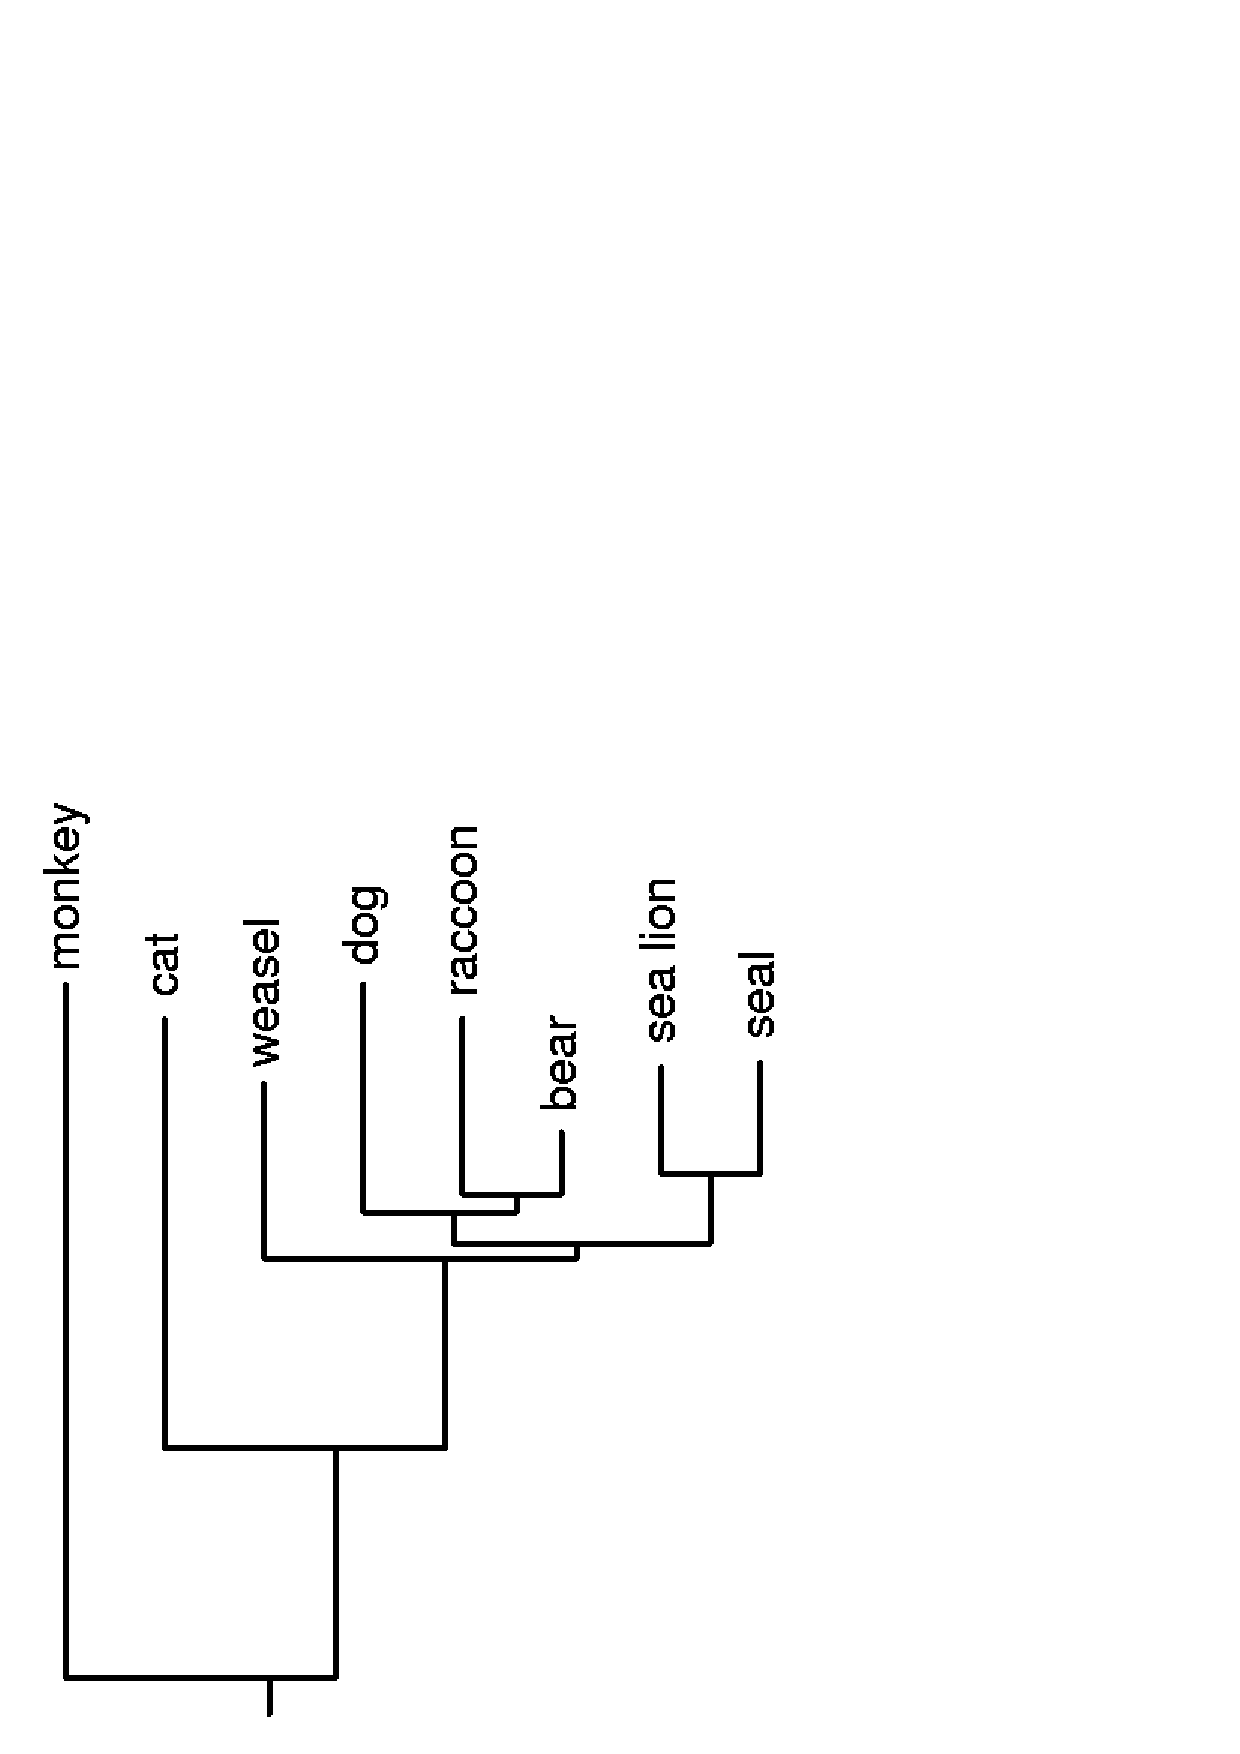
\includegraphics[width=2.2in]{sarichcs.ydraw}}

Same as Neighbor-Joining tree?  Close but not the same.

\end{slide}

\begin{slide}[Replace]{Fitch-Margoliash tree on the Sarich (1969) data}

\centerline{\includegraphics[width=2.2in]{sarichfm.ydraw}}

Same as the unweighted least squares tree?  No.

\end{slide}

\begin{slide}[Replace]{Minimum evolution tree on the Sarich (1969) data}

\centerline{\includegraphics[width=2.2in]{sarichme.ydraw}}

Same as either least squares tree?  As NJ tree?  No.

\end{slide}

\begin{slide}[Replace]{Kimura 2-parameter model}

\centerline{\includegraphics[width=2.4in]{fig13-1.ydraw}}
\bigskip

The simplest, most symmetrical model that has different rates for transitions
than for transversions.

\end{slide}

\begin{slide}[Replace]{Parameters of K2P in terms of Ts/Tn ratio}
\bigskip

If we let $\ \mathsf{R}\ $ be the expected ratio of transition changes to
transversions, it turns out that

{\ptsize{12}
\[
\begin{array}{c c l}
\mathsf{\alpha} & \mathsf{=} & \mathsf{\frac{R}{R+1}}\\
 & & \\
\mathsf{\beta} & \mathsf{=} & \mathsf{\left(\frac{1}{2}\right)\frac{1}{R+1}}
\end{array}
\]
}

\end{slide}

\begin{slide}[Replace]{Transition [sic] probabilities for K2P}
\bigskip

Computing the net probabilities of change (``transition'' in the stochastic
process sense rather than as molecular biologists use it), it turns out that

\[
\begin{array}{l c l}
\mathsf{\prob({\rm transition}|t)} & \mathsf{=} &  \mathsf{\frac{1}{4} - \frac{1}{2} \exp\left(- \frac{2R+1}{R+1}t\right) + \frac{1}{4} \exp\left(-\frac{2}{R+1}t\right)} \\
                                 &   & \\
\mathsf{\prob({\rm transversion}|t)} & \mathsf{=} & \mathsf{\frac{1}{2} - \frac{1}{2} \exp\left(-\frac{2}{R+1}t\right)}.
\end{array}
\]

\end{slide}

\begin{slide}[Replace]{Transition and transversion when $\mathsf{R = 10}$ }
\hspace{0.2in}

\centerline{\includegraphics[width=3.08in]{fig13-2a.ydraw}}

\end{slide}

\begin{slide}[Replace]{Transition and transversion when $\mathsf{R = 2}$ }

\centerline{\includegraphics[width=3.15in]{fig13-2b.ydraw}}

\end{slide}

\begin{slide}[Replace]{ML estimates for the K2P model}
\bigskip

The sufficient statistics for comparison of DNA sequences under the K2P model
are simply the observed fractions $\ \mathsf{P}\ $ and $\ \mathsf{Q}\ $ of
transitions and transversions.  Then the maximum likelihood estimates of the
branch length $\ \mathsf{t}\ $ and of $\ \mathsf{R}\ $ are obtained by finding
the values that predict exactly those fractions.  That done by solving the
equations given three slides ago.

{\ptsize{10}
\[
\begin{array}{c c l}
\mathsf{\widehat{t}} & \mathsf{=} & \mathsf{-\frac{1}{4} \ln \left[(1-2Q)(1-2P-Q)^2 \right]}\\ 
  & & \\
\mathsf{\widehat{R}} & \mathsf{=} & \mathsf{\frac{- \ln (1-2P-Q)}{- \ln (1-2Q)} - \frac{1}{2}}
\end{array} 
\]
}

\end{slide}

\begin{slide}[Replace]{Likelihood for two species under the K2P model}
\bigskip

\noindent
{\ptsize{12}
\[
\begin{array}{c c l}
\mathsf{L} & \mathsf{=} & \mathsf{\prob({\rm data}\, |\, t, R)}\\
& & \\
& \mathsf{=} & \mathsf{\left(\frac{1}{4}\right)^n\;(1-P-Q)^{n-n_1-n_2}\;P^{n_1}\;\left(\frac{1}{2} Q\right)^{n_2}} 
\end{array}
\]
}

\noindent
where $\mathsf{~n_1~}$ is the number of sites differing by transitions, and
$~\mathsf{n_2}~$ is the number of sites differing by transversions.  $~\mathsf{P}~$ and $~\mathsf{Q}~$ are the expected fractions of transition and 
transversion differences, as given by the expressions four screens above.
\bigskip

This is a function of the two parameters $\ \mathsf{t}\ $ and $\ \mathsf{R}\ $.
The values that maximize it were given above, if we estimate both of them.  But
if $\ \mathsf{R}\ $ is given rather than estimated, there is no closed-form
equation solving for $\ \mathsf{t}$, it has to be inferred numerically by
finding the value of $\ \mathsf{t}\ $ that maximizes $\ \mathsf{L}$.

\end{slide}

\begin{slide}[Replace]{The Tamura/Nei model, F84, and HKY}

\begin{displaymath}
\begin{array}{r | c c c c c c c c c c c |}
\cline{2-12}
            {\rm To:} & & ~~~~~~ & A & & G & ~~~~~~ & C & & T & & \\
{\rm From:~}     & & ~~~~~~ &   & &   & ~~~~~~ &   & &   & & \\
\hline
\multicolumn{1}{|c|}{\raisebox{3pt}{\strut}A} & & ~~~~~~ & -       & \multicolumn{3}{r}{\mathsf{\alpha_R \pi_G/\pi_R + \beta \pi_G}}& \mathsf{\beta \pi_C}  & & \mathsf{\beta \pi_T} & & \\
\multicolumn{1}{|c|}{G} & & \multicolumn{3}{l}{\mathsf{\alpha_R \pi_A/\pi_R + \beta \pi_A}} &         -           & ~~~~~~ & \mathsf{\beta \pi_C} & & \mathsf{\beta \pi_T} & & \\
\multicolumn{1}{|c|}{C} & & ~~~~~~ & \mathsf{\beta \pi_A} & & \mathsf{\beta \pi_G} & ~~~~~~ &  - &  \multicolumn{3}{l}{\mathsf{\alpha_Y \pi_T/\pi_Y + \beta \pi_T}} & \\
\multicolumn{1}{|c|}{T} & & ~~~~~~ & \mathsf{\beta \pi_A} & & \mathsf{\beta \pi_G} &\multicolumn{3}{r}{\mathsf{\alpha_Y \pi_C/\pi_Y  + \beta \pi_C}} & - & & \\
\hline
\end{array}
\end{displaymath}
\bigskip

For the F84 model, $~~\mathsf{\alpha_R\ =\ \alpha_Y}$
\bigskip


For the HKY model, $~~\mathsf{\alpha_R/\alpha_Y\ =\ \pi_R/\pi_Y}$

\end{slide}

\begin{slide}[Replace]{Transition/transversion ratio for the Tamura-Nei model}

\[
\begin{array}{c c l}
\mathsf{T_s} & \mathsf{=} & \mathsf{2\;\alpha_R\;\pi_A\;\pi_G\;/\;\pi_R\ +\ 2\;\alpha_Y\;\pi_C\;\pi_T\;/\;\pi_Y}\\
& & \\
& &  \mathsf{+\ \beta\;\left(\;\pi_A\pi_G\;+\;2\pi_C\;\pi_T\right)}\\
& & \\
\mathsf{T_v} & \mathsf{=} & \mathsf{2\;\beta\;\pi_R\;\pi_Y}
\end{array}
\]

To get $\mathsf{~T_s/T_v = R~}$ and $~\mathsf{T_s + T_v = 1}$,

\[
\mathsf{\beta \ = \ \frac{1}{2\pi_R\pi_Y(1+R)}}
\]

\[
\mathsf{\alpha_Y \ = \ \frac{\pi_R\pi_YR - \pi_A\pi_G - \pi_C\pi_T}{(1+R)\left(\pi_Y\pi_A\pi_G\rho + \pi_R\pi_C\pi_T\right)}}
\]

\[
\mathsf{\alpha_R \ = \ \rho\;\alpha_Y}
\]

\end{slide}

\begin{slide}[Replace]{Using fictional events to mimic the Tamura-Nei model}

We imagine two types of events:
\begin{itemize}
\item Type I:
\begin{itemize}
\item If the existing base is a purine, draw a replacement from
a purine pool with bases in relative proportions $~\mathsf{\pi_A\,:\,\pi_G}~$.
This event has rate $~\mathsf{\alpha_R}$.
\item If the existing base is a pyrimidine, draw a replacement from
a pyrimidine pool with bases in relative proportions $~\mathsf{\pi_C\,:\,\pi_T}~$.
This event has rate $~\mathsf{\alpha_Y}$.
\end{itemize}
\medskip

\item Type II: ~~ No matter what the existing base is, replace it by a base
drawn from a pool at the overall equilibrium frequencies:
$~\mathsf{\pi_A\,:\,\pi_C\,:\,\pi_G\,:\,\pi_T}$.  This event has rate
$~\mathsf{\beta}$.
\end{itemize}

\end{slide}

\begin{slide}[Replace]{Transition [sic] probabilities with the Tamura-Nei model}

\begin{center}
\renewcommand{\arraystretch}{1.5}
\begin{tabular}{l l c}
\multicolumn{3}{l}{If the branch starts with a purine:}\\
&No events ~~~ &  $\mathsf{\exp(-(\alpha_R+\beta)t)}$\\
&Some type I, no type II ~~~ &  $\mathsf{\exp(-\beta\;t)\left(1\ -\ \exp(-\alpha_R\;t)\right)}$\\
&Some type II & $\mathsf{1\ -\ \exp(-\beta\;t)}$ \\
& & \\
\multicolumn{3}{l}{If the branch starts with a pyrimidine:}\\
&No events &  $\mathsf{\exp(-(\alpha_Y\;+\;\beta)\;t)}$\\
&Some type I, no type II ~~~ &  $\mathsf{\exp(-\beta\;t)\left(1\ -\ \exp(-\alpha_Y\;t)\right)}$\\
&Some type II & $\mathsf{1\ -\ \exp(-\beta\;t)}$ \\
\end{tabular}
\end{center}

\end{slide}

\begin{slide}[Replace]{A transition probability}

So if we want to compute the probability of getting a G given that a
branch starts with an A, we add up
\begin{itemize}
\item The probability of no events, times 0 (as you can't get a G from an A
with no events)
\item The probability of ``some type I, no type II'' times
$~\mathsf{\pi_G/\pi_Y}~$ (as
the last type I event puts in a G with probability equal to the fraction of
G's out of all purines).
\item The probability of ``some type II'' times $~\mathsf{\pi_G}~$ (as if there is any
type II event, we thereafter have a probability of G equal to its overall
expected frequency, and further type I events don't change that).
\end{itemize}

\end{slide}

\begin{slide}[Replace]{A transition probability}

So that, for example

{\ptsize{12}
\[
\renewcommand{\arraystretch}{1.5}
\begin{array}{l}
\mathsf{\prob(G|A,\;t) \ =}\\
\qquad \mathsf{\exp(-\beta\;t)\;\left(1\ -\ \exp(-\alpha_R\;t)\right)\;\frac{\pi_G}{\pi_R}}\\
\qquad \mathsf{+ \ \left(1\  -\  \exp(-\beta\;t)\right)\;\pi_G }
\end{array}
\]
}

\end{slide}

\begin{slide}[Replace]{A more compact expression}

More generally, we can use the Kronecker delta notation $\mathsf{~\delta_{ij}~}$
and the ``Watson-Kronecker'' notation $\mathsf{~\varepsilon_{ij}~}$ to write

{\ptsize{12}
\[
\begin{array}{l}
\mathsf{\prob(j\, |\, i, t) \ =}\\
\qquad  \mathsf{\exp(-(\alpha_i+\beta)t)\;\delta_{ij}}\\
\qquad  \mathsf{+ \exp(-\beta t)\left(1 - \exp(-\alpha_it)\right) \left(\frac{\pi_j \varepsilon_{ij}}{\sum_k \varepsilon_{jk}\pi_k} \right)}\\
\qquad  \mathsf{+ \left(1 - \exp(-\beta t)\right) \pi_j}
\end{array}
\]
}
\bigskip

where $\delta_{ij}$ is 1 if the two bases $i$ and $j$ are different (0 otherwise),

and $\varepsilon_{ij}$ is 1 if, of the two bases $i$ and $j$, one is a purine and
one is a pyrimidine (0 otherwise).

\end{slide}

\begin{slide}[Replace]{Reversibility and the GTR model}
\bigskip

The condition of {\it reversibility} in a stochastic process is written in
terms of the equilibrium frequences of the states ($\ \mathsf{\pi_i}\ $ and
the transition probabilities as

\[
\mathsf{\pi_i\;\prob(j | i, t)\ =\ \pi_j\;\prob(i | j, t)}
\]
\bigskip

The general time-reversible model:

\[\begin{array}{c c | c c c c |}
\cline{3-6}
 & {\rm To:} & A & G & C & T \\ 
{\rm From:} & & & & & \\
\hline
\multicolumn{2}{|c|}{A} & {\rm\raisebox{3pt}{\strut} -} & \mathsf{\pi_G\;\alpha} & \mathsf{\pi_C\;\beta} & \mathsf{\pi_T\;\gamma} \\
\multicolumn{2}{|c|}{G} & \mathsf{\pi_A\;\alpha} & {\rm -} & \mathsf{\pi_C\;\delta} & \mathsf{\pi_T\;\varepsilon} \\
\multicolumn{2}{|c|}{C} & \mathsf{\pi_A\;\beta} & \mathsf{\pi_G\;\delta} & {\rm -} & \mathsf{\pi_T\;\eta} \\
\multicolumn{2}{|c|}{T} & \mathsf{\pi_A\;\gamma} & \mathsf{\pi_G\;\varepsilon} & \mathsf{\pi_C\;\eta} & {\rm -}\\
\hline
\end{array}
\]

\end{slide}

\begin{slide}[Replace]{The GTR model}

\centerline{\includegraphics[width=2.5in]{gtr.ydraw}}
\bigskip

It is the most general model possible that still has the changes satisfy the
condition of reversibility -- so that one cannot tell which direction evolution
has gone by examining the sequences before and after.

\end{slide}

\begin{slide}[Replace]{Standardizing the rates}
\bigskip

{\ptsize{12}
\[
\begin{array}{l}
\mathsf{2\pi_A\;\pi_G\;\alpha\ +\ 2\;\pi_A\;\pi_C\;\beta\ +\ 2\;\pi_A\;\pi_T\;\gamma}\\
\\
 \mathsf{+\ 2\;\pi_G\;\pi_C\;\delta\ +\ 2\;\pi_G\;\pi_T\;\varepsilon\ +\ 2\;\pi_C\;\pi_T\;\eta\ =\ 1}
\end{array}
\]
}
\bigskip

This is done so that the expected rate of change is $\ \mathsf{1}\ $ per unit
time.

\end{slide}

\begin{slide}[Replace]{General Time Reversible models -- inference}

\centerline{A data example (simulated under a K2P model, true distance 0.2}
\centerline{transition/transversion ratio = 2}

\begin{center} 
\[
\renewcommand{\arraystretch}{1.4}
\begin{array}{c | c c c c | c} 
     & {\tt A} & {\tt G} & {\tt C} & {\tt T} & {\rm total} \\
\hline
{\tt A \raisebox{3pt}{\strut}} & \mathsf{93} & \mathsf{13} & \mathsf{3} & \mathsf{3} & \mathsf{112}\\
{\tt G} & \mathsf{10} & \mathsf{105} & \mathsf{3} & \mathsf{4} & \mathsf{122}\\
{\tt C} & \mathsf{6} & \mathsf{4} & \mathsf{113} & \mathsf{18} & \mathsf{141}\\
{\tt T} & \mathsf{7} & \mathsf{4} & \mathsf{21} & \mathsf{93} & \mathsf{125}\\
\hline
{\rm total} & \mathsf{116} & \mathsf{126} & \mathsf{140} & \mathsf{118} & \mathsf{500}
\end{array}
\]
\end{center}
\bigskip

The K2P model is a special case of the GTR model (as are all the other models
that have been mentioned here).  So if all goes well we should infer parameters
that come close to specifying a K2P model.

\end{slide}

\begin{slide}[Replace]{Averaging across the diagonal ... }

\begin{center}
\[
\renewcommand{\arraystretch}{1.3}
\begin{array}{c | c c c c | c}
     & {\tt A} & {\tt G} & {\tt C} & {\tt T} & {\rm total} \\
\hline
{\tt A} & \mathsf{93} & \mathsf{11.5} & \mathsf{4.5} & \mathsf{5} & \mathsf{114}\\
{\tt G} & \mathsf{11.5} & \mathsf{105} & \mathsf{3.5} & \mathsf{4} & \mathsf{124}\\
{\tt C} & \mathsf{4.5} & \mathsf{3.5} & \mathsf{113} & \mathsf{19.5} & \mathsf{140.5}\\
{\tt T} & \mathsf{5} & \mathsf{4} & \mathsf{19.5} & \mathsf{93} & \mathsf{121.5}\\
\hline
{\rm total} & \mathsf{114} & \mathsf{124} & \mathsf{140.5} & \mathsf{121.5} & \mathsf{500}
\end{array}
\]
\end{center}

\end{slide}

\begin{slide}[Replace]{Dividing each column by its sum}

(column, because $\mathsf{~P_{ij}~}$ is to be the
probability of change from $~\mathsf{j}~$ to $~\mathsf{i}~$)

\[
\renewcommand{\arraystretch}{1.3}
\mathsf{\hat{\bf P} = \left[
\begin{array}{l l l l}
\mathsf{0.815789} & \mathsf{0.0927419} & \mathsf{0.0320285} & \mathsf{0.0411523}\\
\mathsf{0.100877} & \mathsf{0.846774} & \mathsf{0.024911} & \mathsf{0.0329218}\\
\mathsf{0.0394737} & \mathsf{0.0282258} & \mathsf{0.80427} & \mathsf{0.160494}\\
\mathsf{0.0438596} & \mathsf{0.0322581} & \mathsf{0.13879} & \mathsf{0.765432}
\end{array}
\right]
}
\]

\end{slide}

\begin{slide}[Replace]{Rate matrix from the matrix logarithm}

If the rate matrix is $~\mathsf{{\bf A}}$,

\[
\mathsf{{\bf P} \ = \ e^{{\bf A}\,t}}
\]

so that

\[
\renewcommand{\arraystretch}{1.3}
\begin{array}{c c l}
\mathsf{\widehat{{\bf A}t}} & \mathsf{=} & \mathsf{\log \left(\hat{\bf P}\right)} \\
& & \\
& \mathsf{=}  &\mathsf{\left[
\begin{array}{l l l l} 
\mathsf{-0.212413} & \mathsf{0.110794} & \mathsf{0.034160} & \mathsf{0.046726}\\
\mathsf{0.120512} & \mathsf{-0.174005} & \mathsf{0.025043} & \mathsf{0.035554}\\
\mathsf{0.0421002} & \mathsf{0.028375} & \mathsf{-0.236980} & \mathsf{0.205579}\\
\mathsf{0.0498001} & \mathsf{0.034837} & \mathsf{0.177778} & \mathsf{-0.287859}\\
\end{array} 
\right].
}
\end{array}
\]

\end{slide}

\begin{slide}[Replace]{Standardizing the rates}

If we denote by $~\mathsf{\hat{\bf D}}~$ the diagonal matrix of observed base frequencies,
and we require that the rate of (potentially-observable)
substitution is 1:

\[
\mathsf{- {\rm trace} ({\bf \hat{A} \hat{D}}) = 1}
\]

We get:
\[
\mathsf{\hat{t} = - {\rm trace} (\widehat{{\bf A}t} \hat{\bf D}) = - {\rm trace} \left(\log (\hat{\bf P})\hat{\bf D}\right)}
\]

and that also gives us an estimate of the rate matrix:
\[
\mathsf{\hat{\bf A} =  \log \left(\hat{\bf P}\right) \big/ - {\rm trace} \left(\log (\hat{\bf P})\hat{\bf D}\right)}
\]

\end{slide}

\begin{slide}[Replace]{The rate estimates}

\[
\renewcommand{\arraystretch}{1.3}
\mathsf{\hat{\bf A} = \left[
\begin{array}{r r r r}
\mathsf{-0.931124} & \mathsf{0.485671} & \mathsf{0.149741} & \mathsf{0.204826}\\
\mathsf{0.528274} & \mathsf{-0.762764} & \mathsf{0.109776} & \mathsf{0.155852}\\
\mathsf{0.184549} & \mathsf{0.124383} & \mathsf{-1.038820} & \mathsf{0.901168}\\
\mathsf{0.218302} & \mathsf{0.152710} & \mathsf{0.779302} & \mathsf{-1.261850}\\
\end{array}
\right].
}
\]

moderately close to the actual K2P rate matrix used in the
simulation which was:

\[
\renewcommand{\arraystretch}{1.3}
\mathsf{{\bf A} = \left[
\begin{array}{c c c c}
\mathsf{-1} & \mathsf{2/3} & \mathsf{1/6} & \mathsf{1/6}\\
\mathsf{2/3} & \mathsf{-1} & \mathsf{1/6} & \mathsf{1/6}\\
\mathsf{1/6} & \mathsf{1/6} & \mathsf{-1} & \mathsf{2/3}\\
\mathsf{1/6} & \mathsf{1/6} & \mathsf{2/3} & \mathsf{-1}
\end{array}
\right]
}
\]

(but if any of the eigenvalues of $~\mathsf{\log(\hat{\bf P})}~$ are negative, this doesn't
work and the divergence time is estimated to be infinite).

\end{slide}

\begin{slide}[Replace]{The lattice of these models}

\centerline{\includegraphics[width=1.6in]{modellattice.ydraw}}
\bigskip

There are a great many other models, but these are the most commonly used.
They allow for unequal expected frequencies of bases, and for
inequalities of transitions and transversions.

\end{slide}

\end{document}

